\chapter{Resultados}
\label{chap_resultados}

Neste capítulo, são apresentados os resultados de simulação gerados pelo executável desenvolvido para o projeto. As figuras apresentam a evolução espaço-temporal com tempo crescente para baixo (\(t=0\) no topo), seguindo a convenção utilizada na literatura de ECA.
Essa mesma convenção foi adotada na interface Python do executável, mantendo consistência entre a visualização da aplicação e as figuras deste relatório.
As conclusões desta seção são qualitativas e baseadas nas imagens geradas durante a execução do aplicativo.

\section{Regras representativas por classe}

As Figuras~\ref{fig:homogeneo-r0} a~\ref{fig:complexo-r110} mostram duas regras por classe de Wolfram. Em todos os casos, os parâmetros foram: \(tamanho=101\), \(passos=120\), estado inicial central, densidade \(0{,}5\) e agrupado = nao.

\begin{table}[H]
\centering
\caption{Regras selecionadas por classe para atendimento ao roteiro da prática.}
\label{tab:regras-classes}
\begin{tabular}{ll}
\toprule
Classe & Regras utilizadas \\
\midrule
Homogênea & 0, 255 \\
Periódica & 4, 108 \\
Caótica & 30, 90 \\
Complexa & 54, 110 \\
\bottomrule
\end{tabular}
\end{table}

\begin{figure}[H]
    \centering
    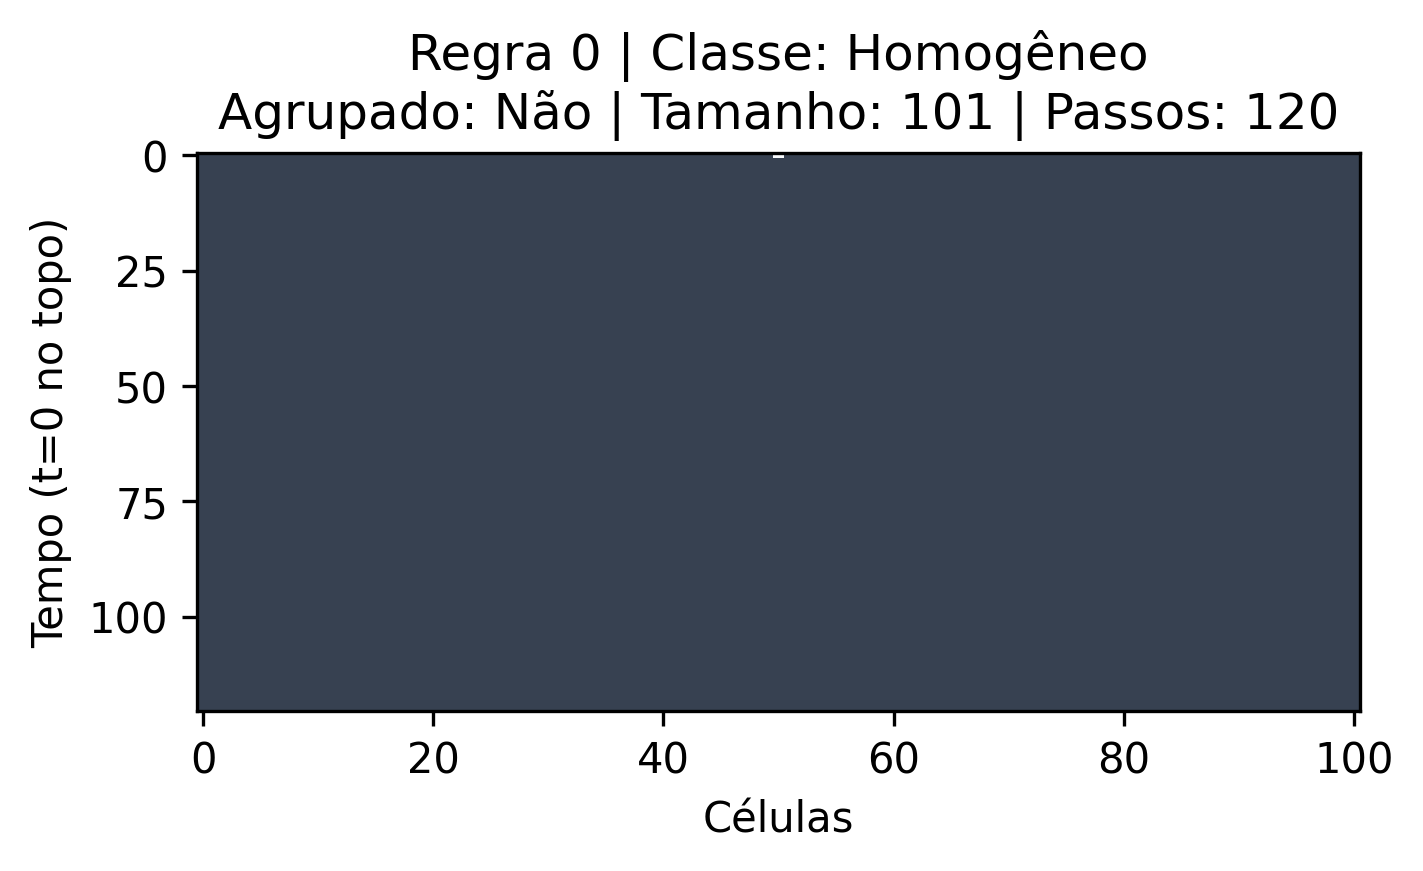
\includegraphics[width=0.75\textwidth]{figuras/resultados/regra_0_tamanho_101_passos_120_estado_central_densidade_0_5_agrupado_nao_classe_homogeneo.png}
    \caption{Classe homogênea, Regra 0 (tam101, passos120, estado central, dens05, agrupado nao).}
    \label{fig:homogeneo-r0}
\end{figure}

\begin{figure}[H]
    \centering
    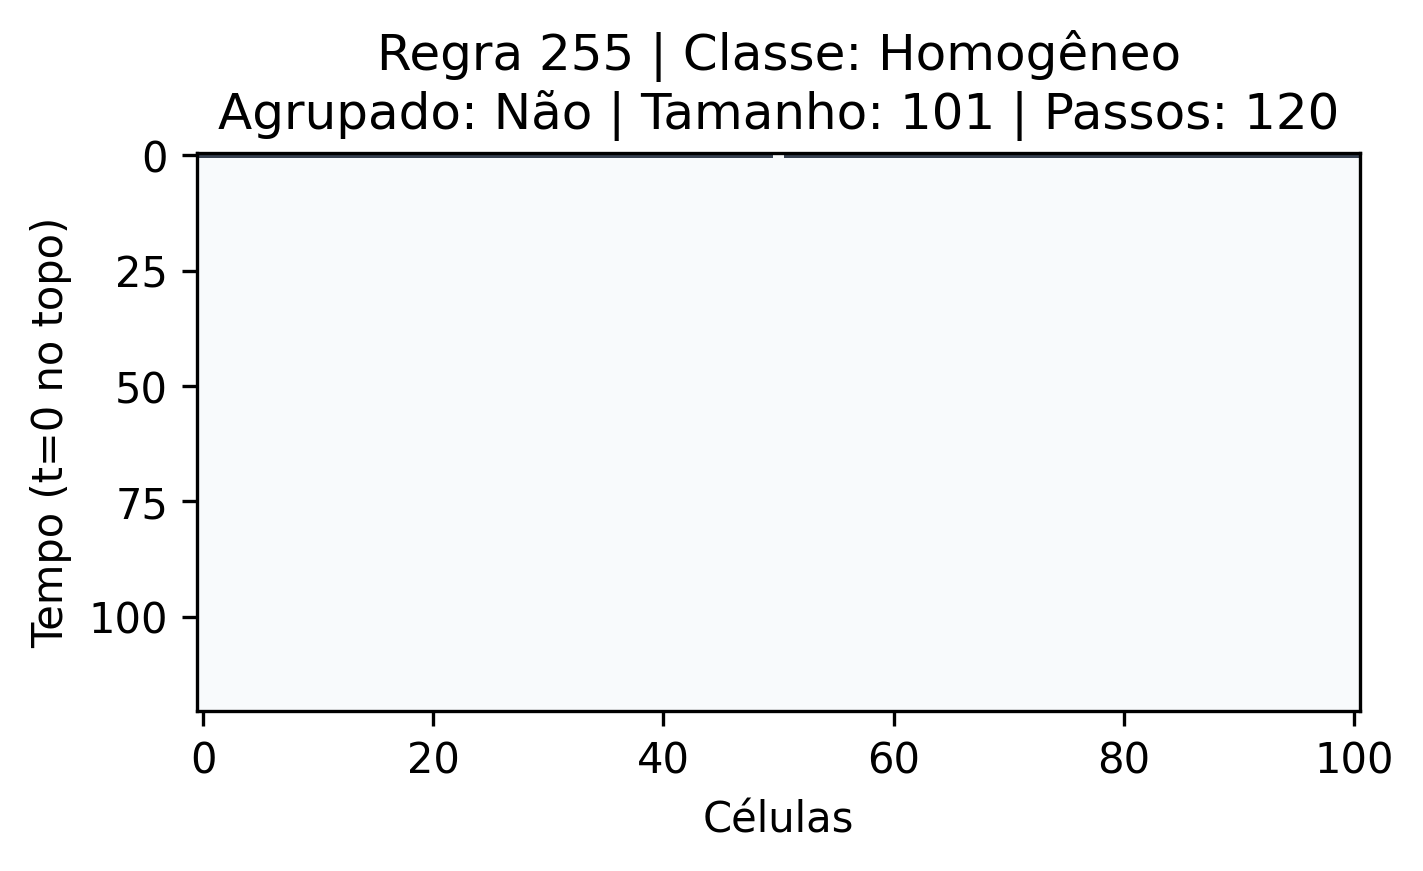
\includegraphics[width=0.75\textwidth]{figuras/resultados/regra_255_tamanho_101_passos_120_estado_central_densidade_0_5_agrupado_nao_classe_homogeneo.png}
    \caption{Classe homogênea, Regra 255 (tam101, passos120, estado central, dens05, agrupado nao).}
    \label{fig:homogeneo-r255}
\end{figure}

\begin{figure}[H]
    \centering
    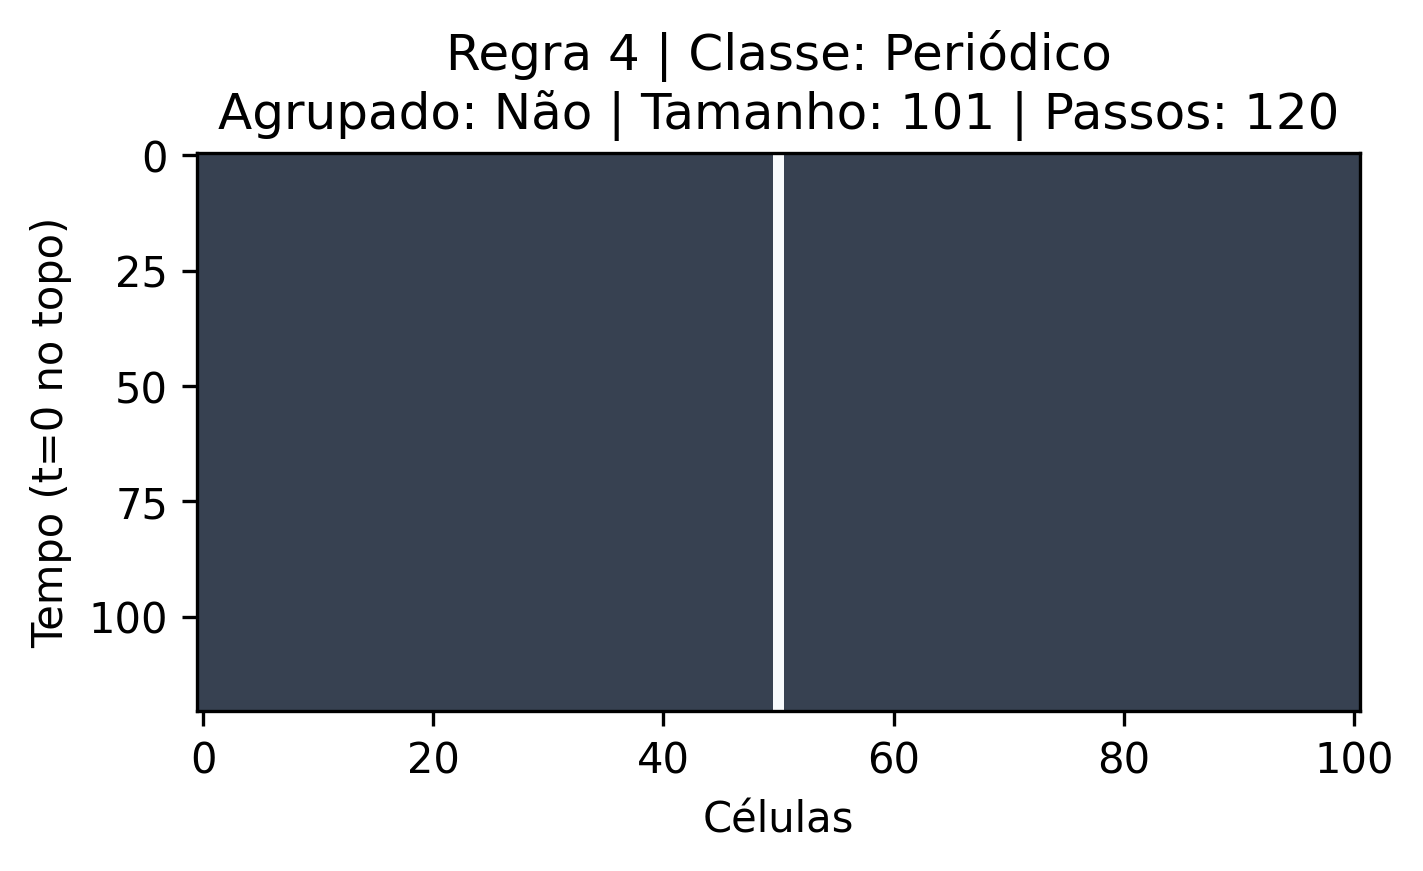
\includegraphics[width=0.75\textwidth]{figuras/resultados/regra_4_tamanho_101_passos_120_estado_central_densidade_0_5_agrupado_nao_classe_periodico.png}
    \caption{Classe periódica, Regra 4 (tam101, passos120, estado central, dens05, agrupado nao).}
    \label{fig:periodico-r4}
\end{figure}

\begin{figure}[H]
    \centering
    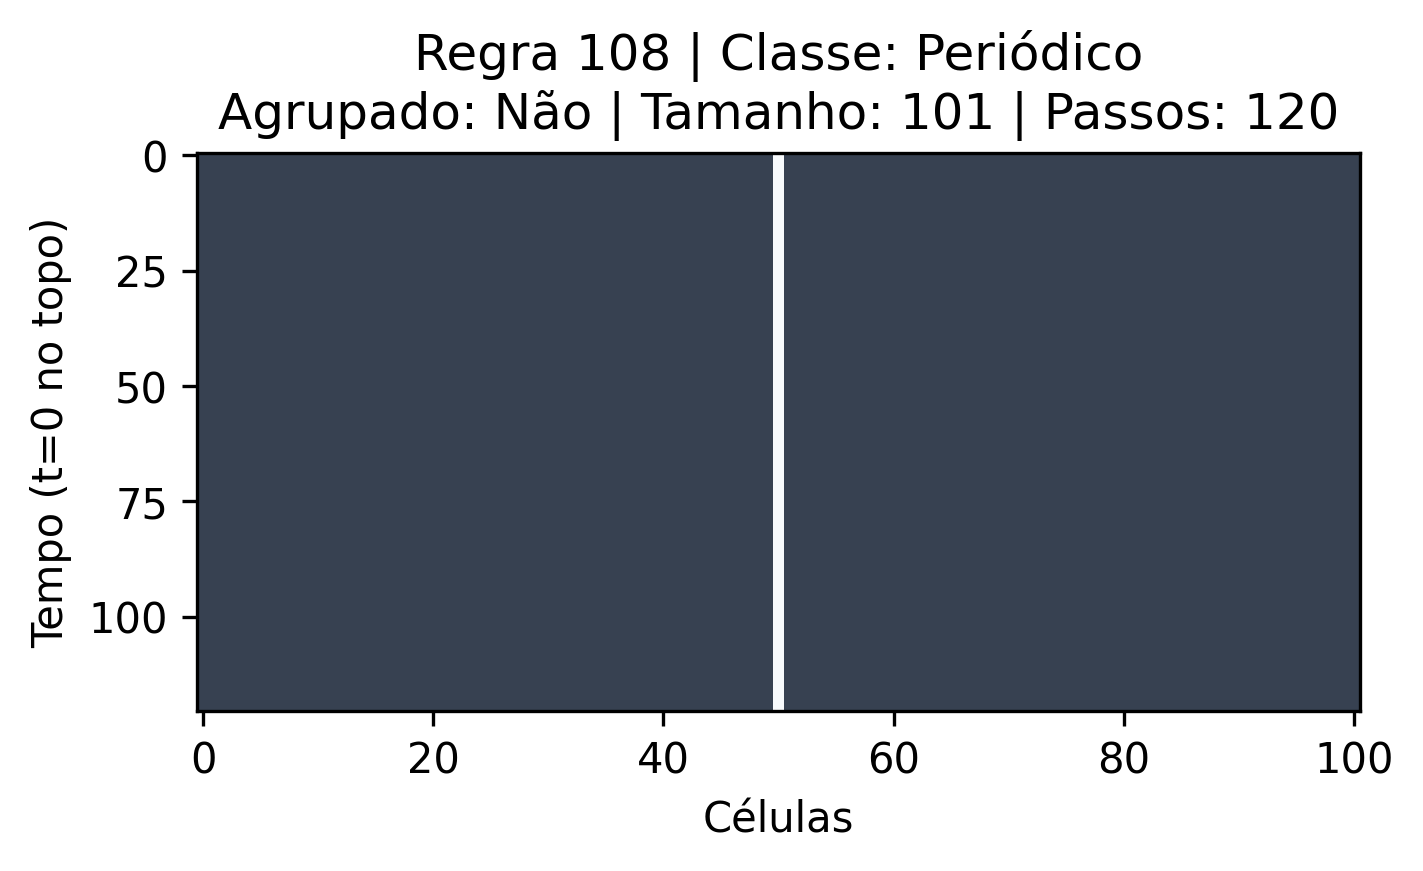
\includegraphics[width=0.75\textwidth]{figuras/resultados/regra_108_tamanho_101_passos_120_estado_central_densidade_0_5_agrupado_nao_classe_periodico.png}
    \caption{Classe periódica, Regra 108 (tam101, passos120, estado central, dens05, agrupado nao).}
    \label{fig:periodico-r108}
\end{figure}

\begin{figure}[H]
    \centering
    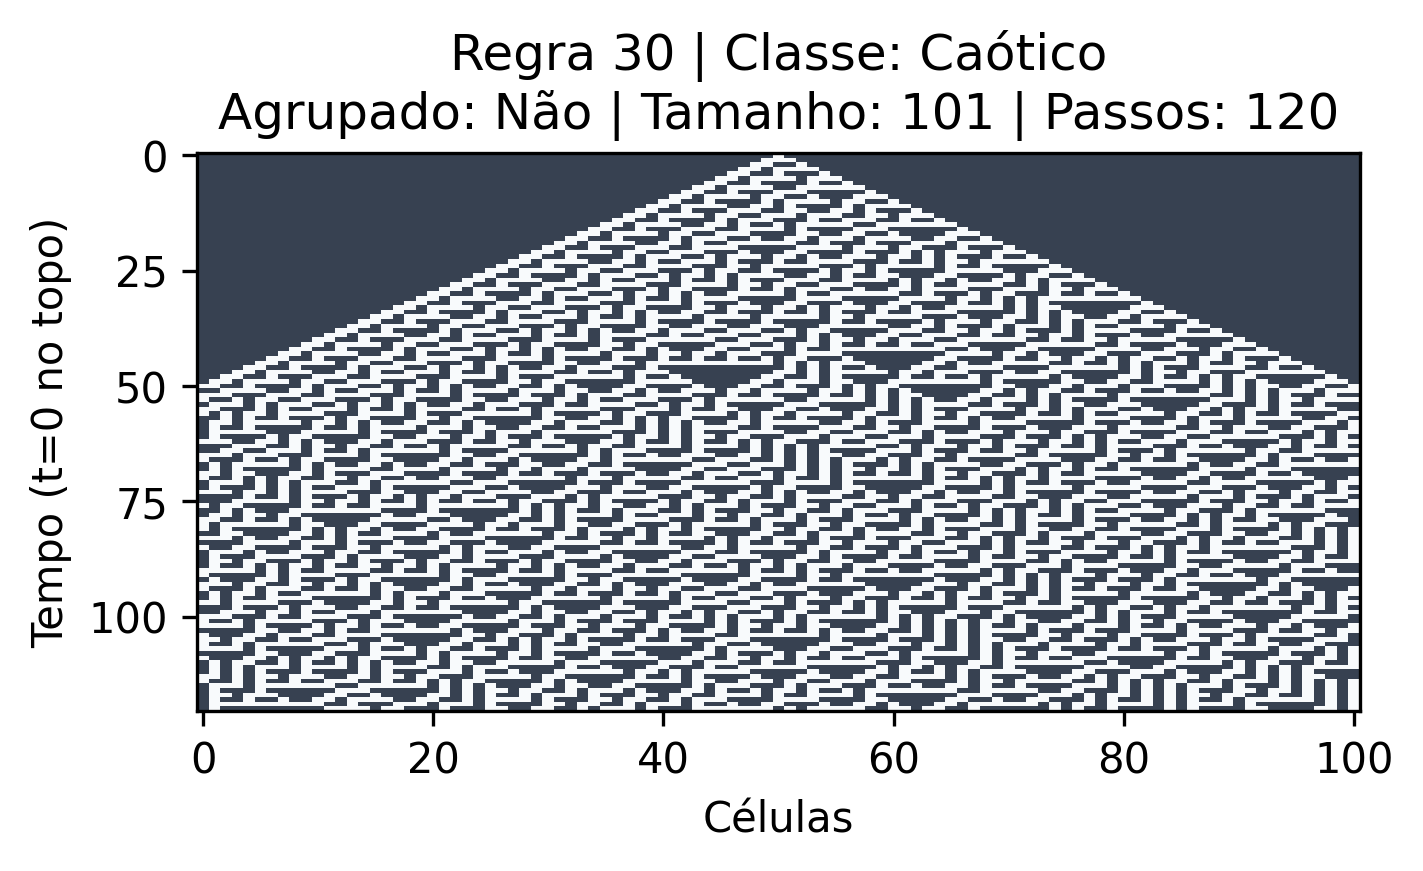
\includegraphics[width=0.75\textwidth]{figuras/resultados/regra_30_tamanho_101_passos_120_estado_central_densidade_0_5_agrupado_nao_classe_caotico.png}
    \caption{Classe caótica, Regra 30 (tam101, passos120, estado central, dens05, agrupado nao).}
    \label{fig:caotico-r30}
\end{figure}

\begin{figure}[H]
    \centering
    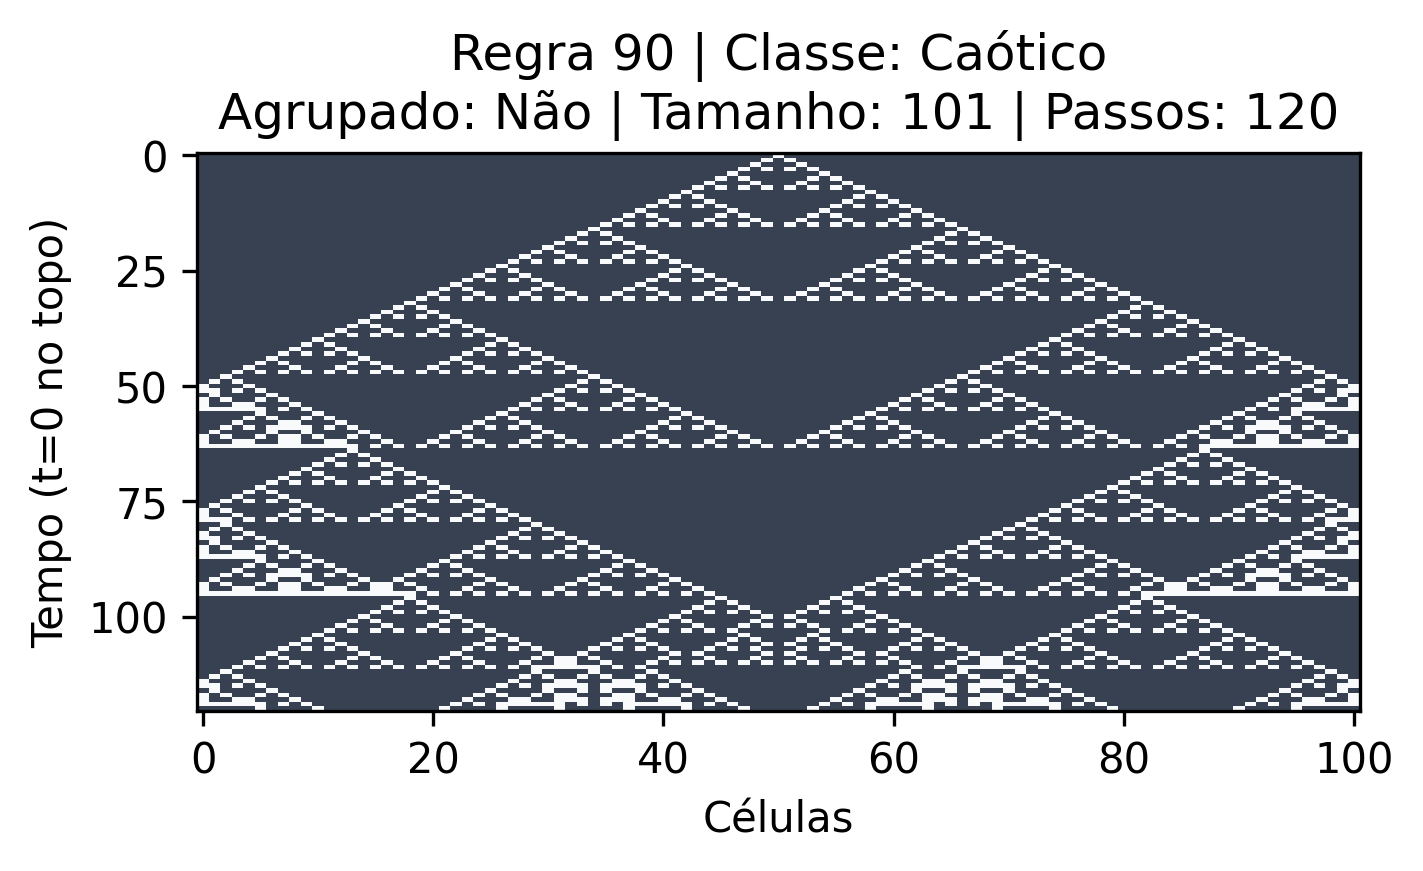
\includegraphics[width=0.75\textwidth]{figuras/resultados/regra_90_tamanho_101_passos_120_estado_central_densidade_0_5_agrupado_nao_classe_caotico.png}
    \caption{Classe caótica, Regra 90 (tam101, passos120, estado central, dens05, agrupado nao).}
    \label{fig:caotico-r90}
\end{figure}

\begin{figure}[H]
    \centering
    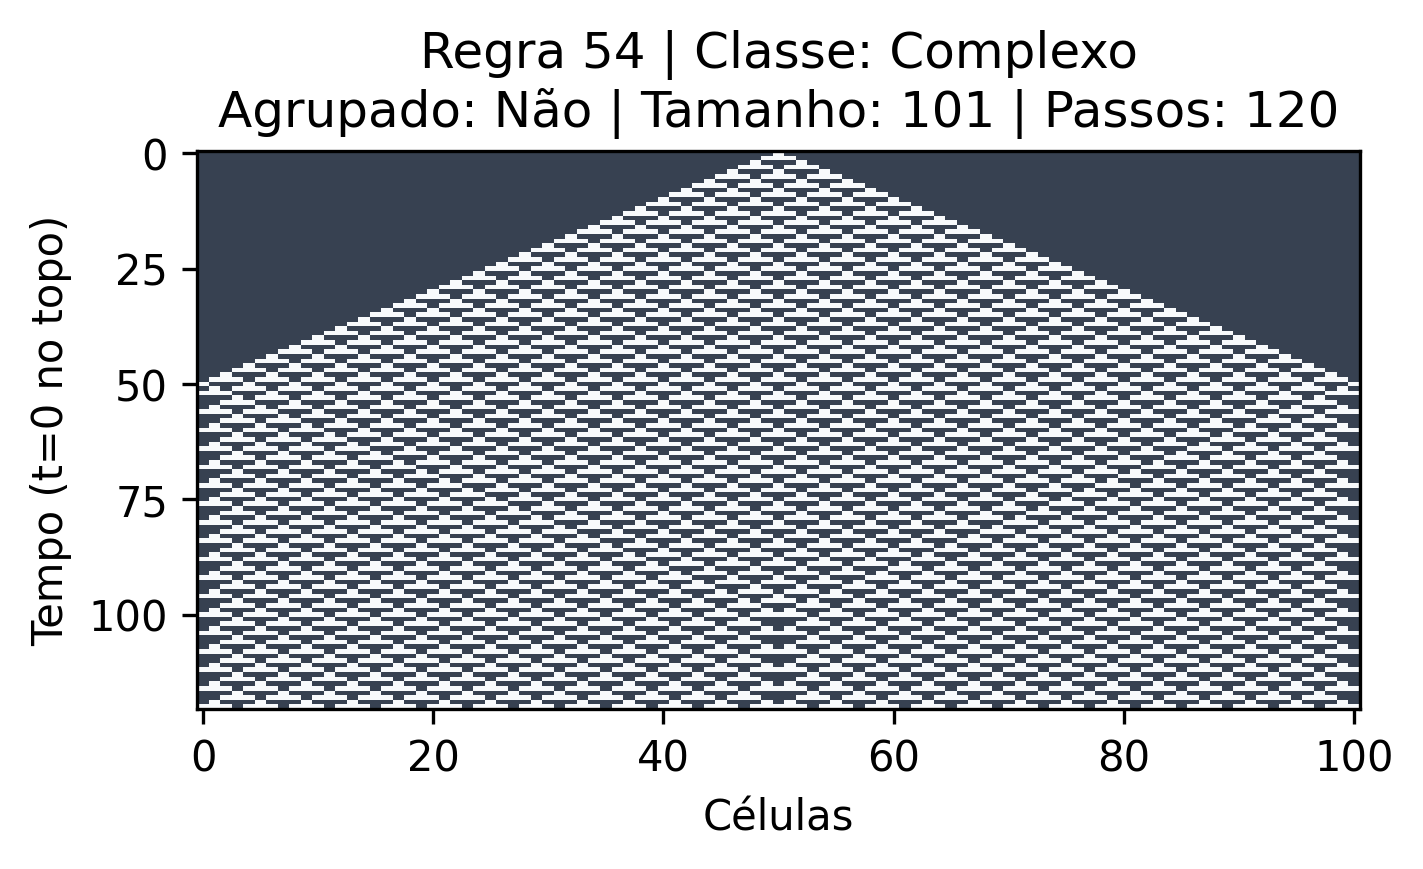
\includegraphics[width=0.75\textwidth]{figuras/resultados/regra_54_tamanho_101_passos_120_estado_central_densidade_0_5_agrupado_nao_classe_complexo.png}
    \caption{Classe complexa, Regra 54 (tam101, passos120, estado central, dens05, agrupado nao).}
    \label{fig:complexo-r54}
\end{figure}

\begin{figure}[H]
    \centering
    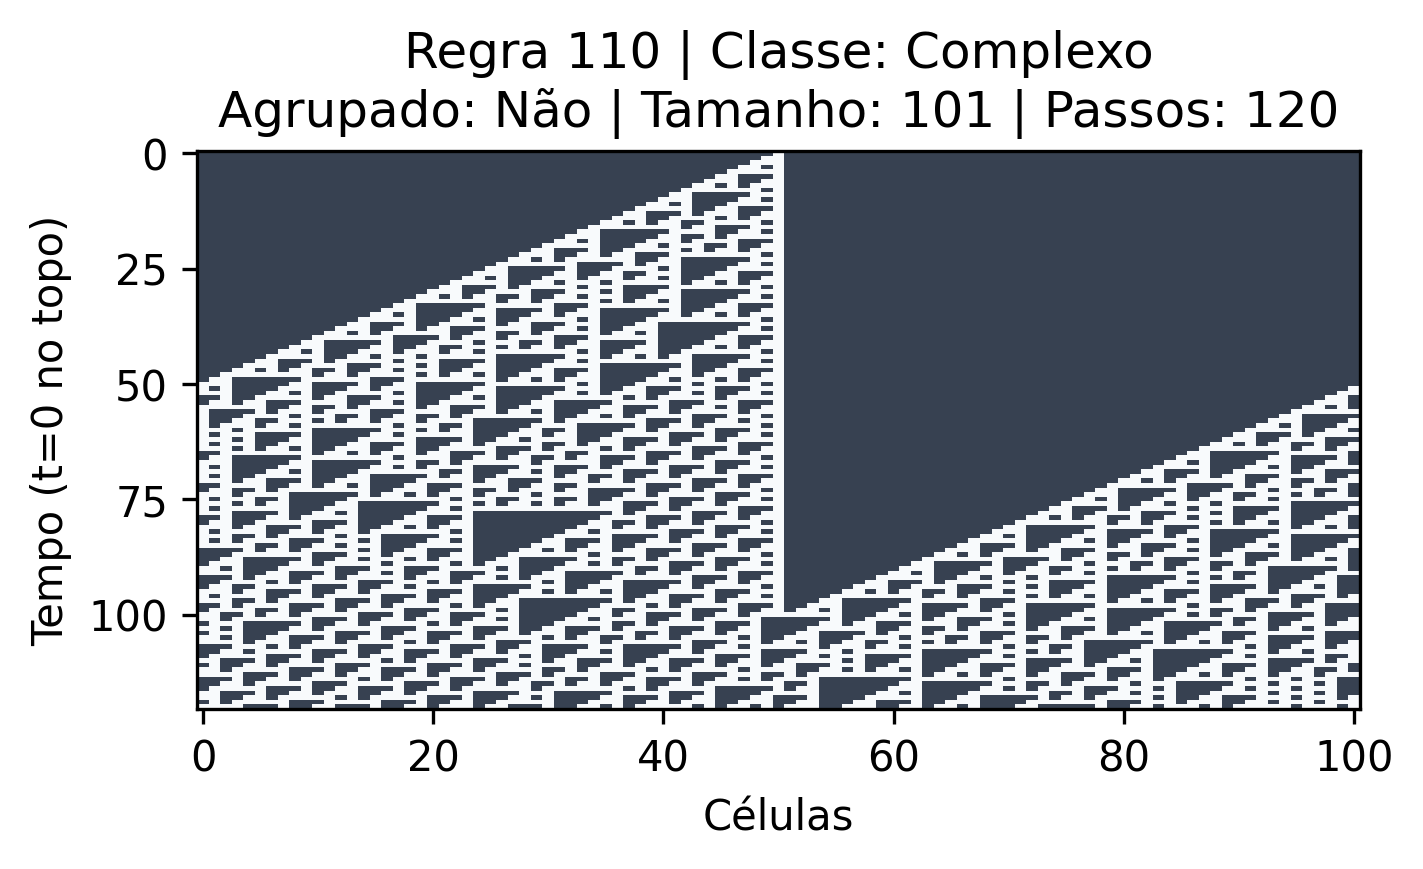
\includegraphics[width=0.75\textwidth]{figuras/resultados/regra_110_tamanho_101_passos_120_estado_central_densidade_0_5_agrupado_nao_classe_complexo.png}
    \caption{Classe complexa, Regra 110 (tam101, passos120, estado central, dens05, agrupado nao).}
    \label{fig:complexo-r110}
\end{figure}

A classificação visual é coerente com a literatura: as regras 0 e 255 convergem para padrões homogêneos (Figuras~\ref{fig:homogeneo-r0} e~\ref{fig:homogeneo-r255}); as regras 4 e 108 apresentam regularidade periódica (Figuras~\ref{fig:periodico-r4} e~\ref{fig:periodico-r108}); as regras 30 e 90 exibem comportamento irregular típico de classe caótica (Figuras~\ref{fig:caotico-r30} e~\ref{fig:caotico-r90}); e as regras 54 e 110 mostram coexistência de estruturas locais com interações não triviais, caracterizando classe complexa (Figuras~\ref{fig:complexo-r54} e~\ref{fig:complexo-r110}) \cite{wolfram2002,wikipediaECA,wolframAtlas}.

\section{Comparações adicionais com estado aleatório e densidade}

Para complementar a análise, também foram incluídos experimentos com estado inicial aleatório e variação de densidade, mantendo \(tamanho=101\), \(passos=120\) e agrupado = nao.

\begin{figure}[H]
    \centering
    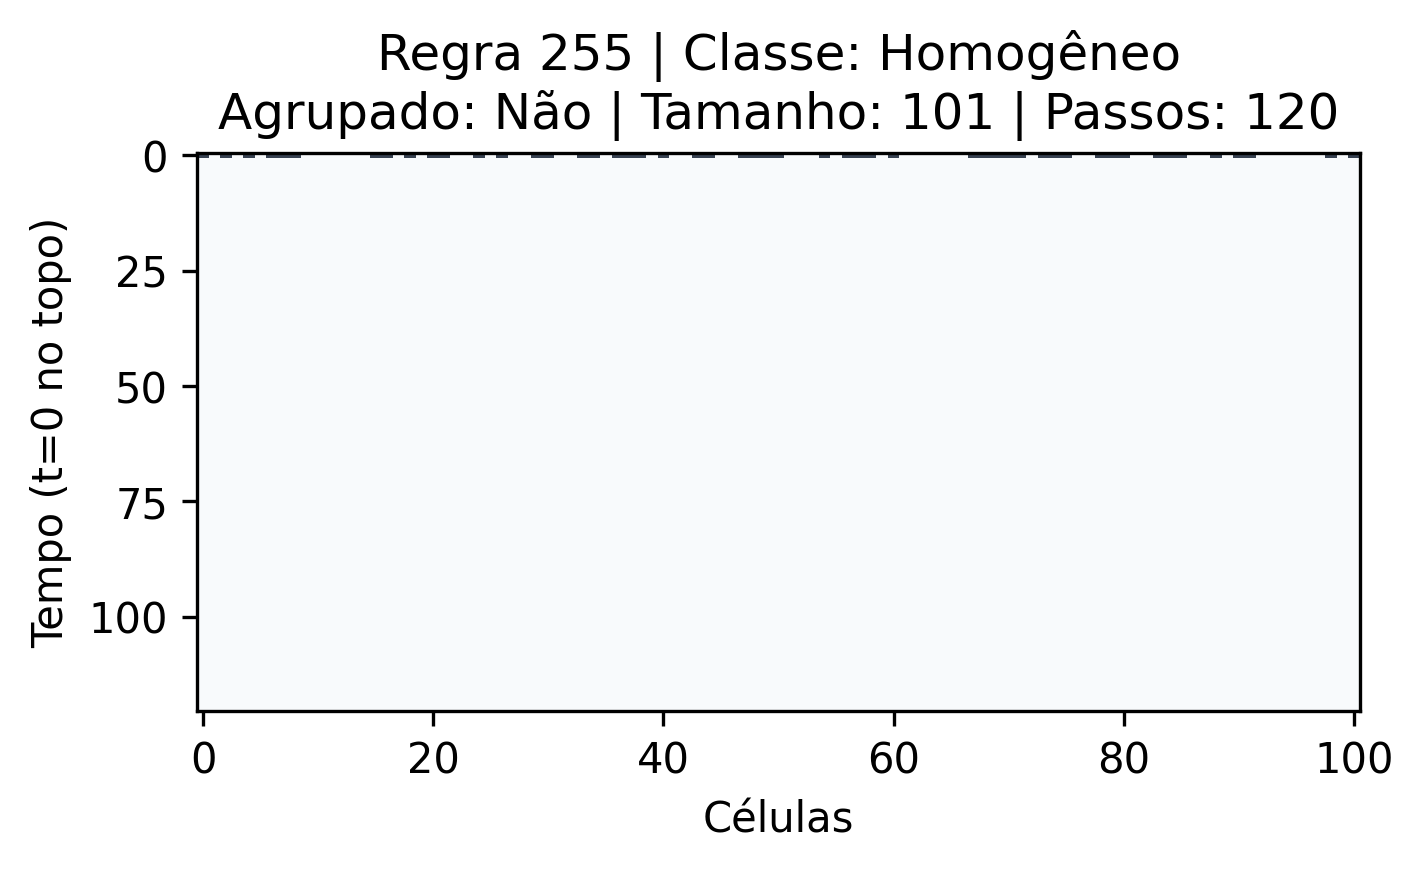
\includegraphics[width=0.75\textwidth]{figuras/resultados/regra_255_tamanho_101_passos_120_estado_aleatorio_densidade_0_5_agrupado_nao_classe_homogeneo.png}
    \caption{Regra 255 com estado aleatório e densidade 0,5.}
    \label{fig:extra-r255-a05}
\end{figure}

\begin{figure}[H]
    \centering
    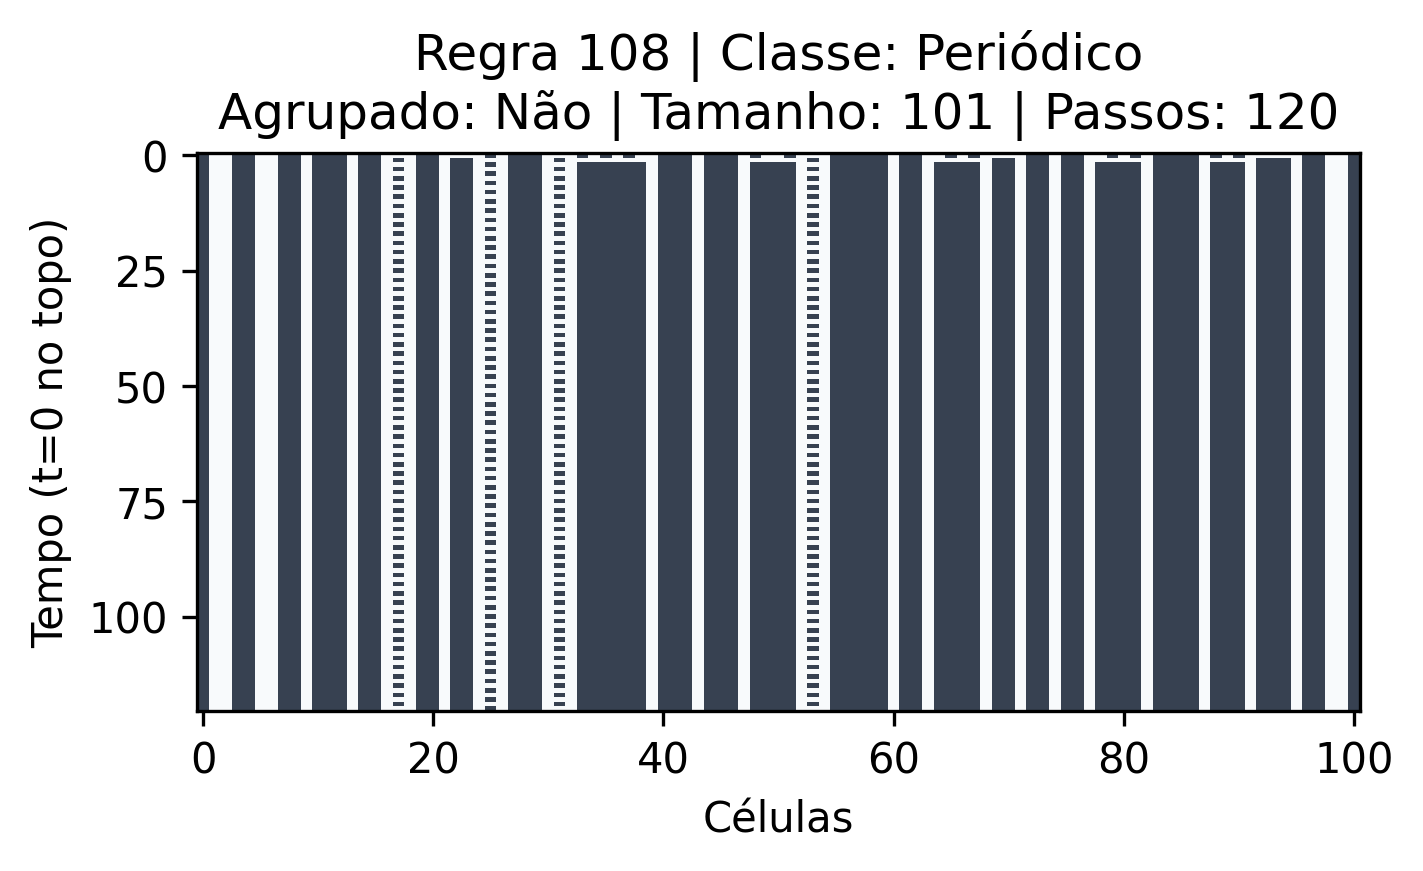
\includegraphics[width=0.75\textwidth]{figuras/resultados/regra_108_tamanho_101_passos_120_estado_aleatorio_densidade_0_5_agrupado_nao_classe_periodico.png}
    \caption{Regra 108 com estado aleatório e densidade 0,5.}
    \label{fig:extra-r108-a05}
\end{figure}

\begin{figure}[H]
    \centering
    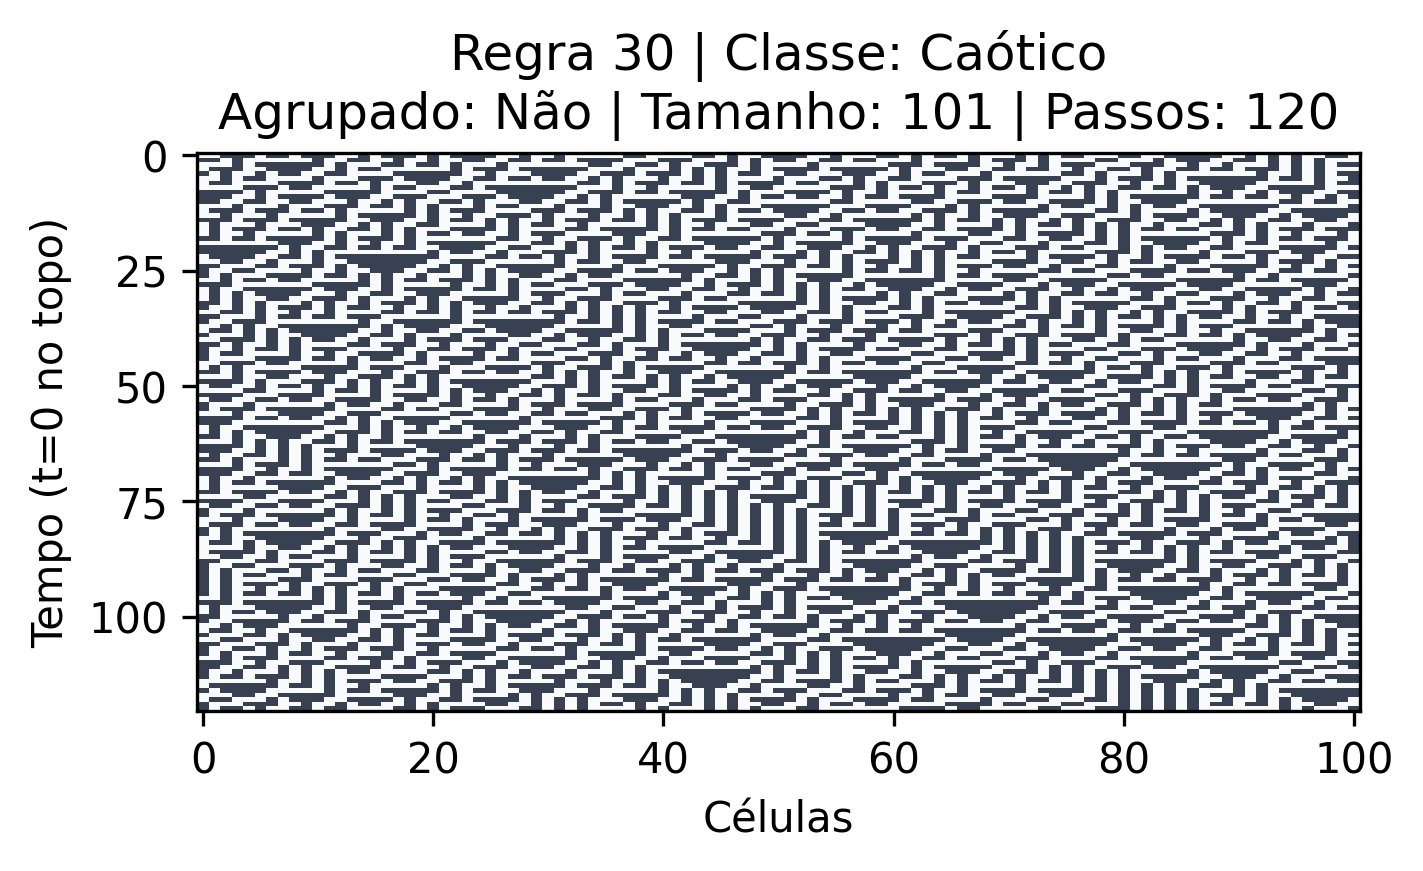
\includegraphics[width=0.75\textwidth]{figuras/resultados/regra_30_tamanho_101_passos_120_estado_aleatorio_densidade_0_5_agrupado_nao_classe_caotico.png}
    \caption{Regra 30 com estado aleatório e densidade 0,5.}
    \label{fig:extra-r30-a05}
\end{figure}

\begin{figure}[H]
    \centering
    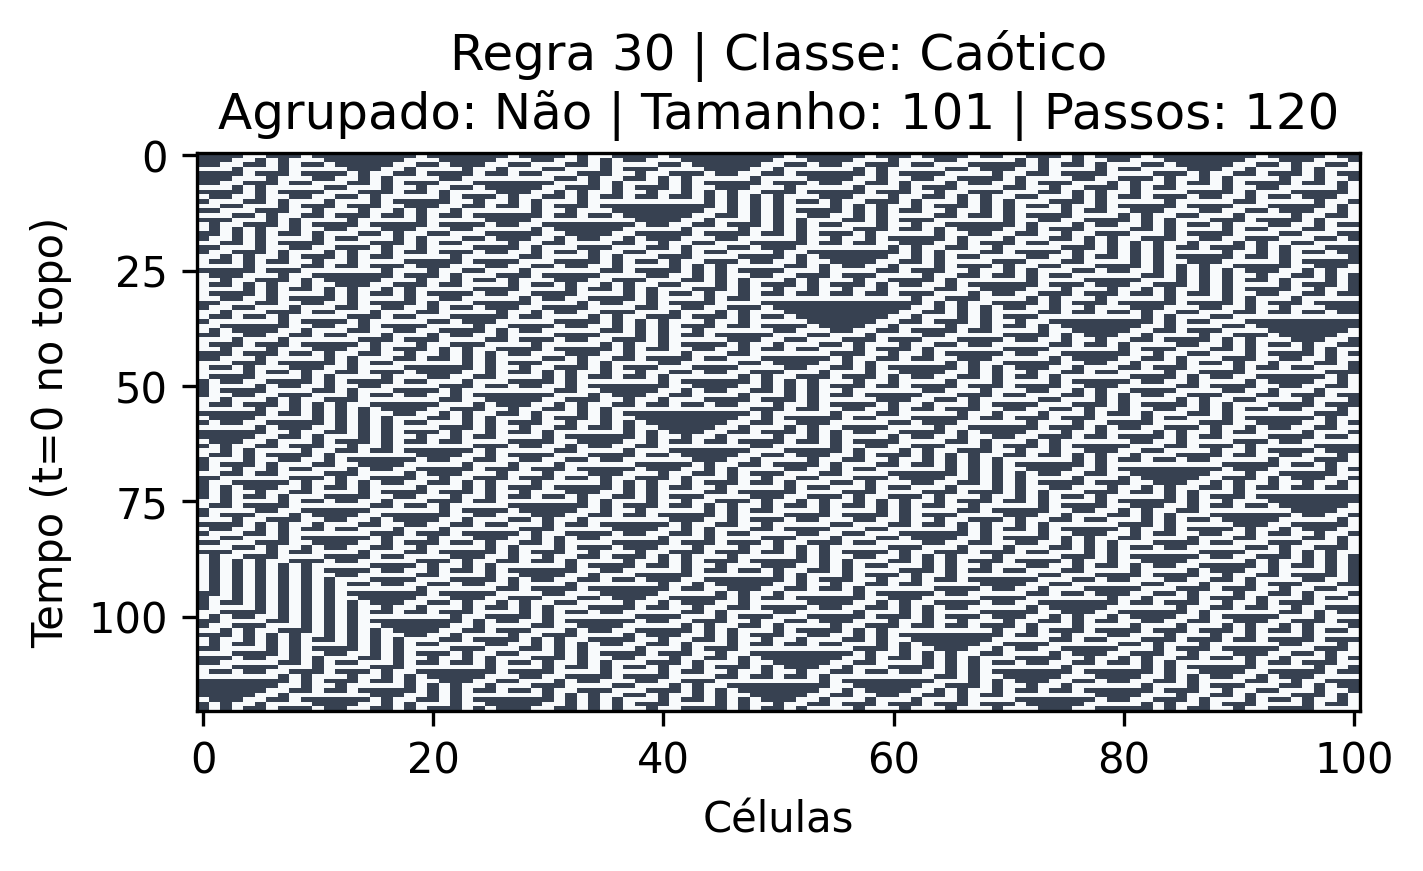
\includegraphics[width=0.75\textwidth]{figuras/resultados/regra_30_tamanho_101_passos_120_estado_aleatorio_densidade_0_2_agrupado_nao_classe_caotico.png}
    \caption{Regra 30 com densidade 0,2 (estado aleatório).}
    \label{fig:extra-r30-a02}
\end{figure}

\begin{figure}[H]
    \centering
    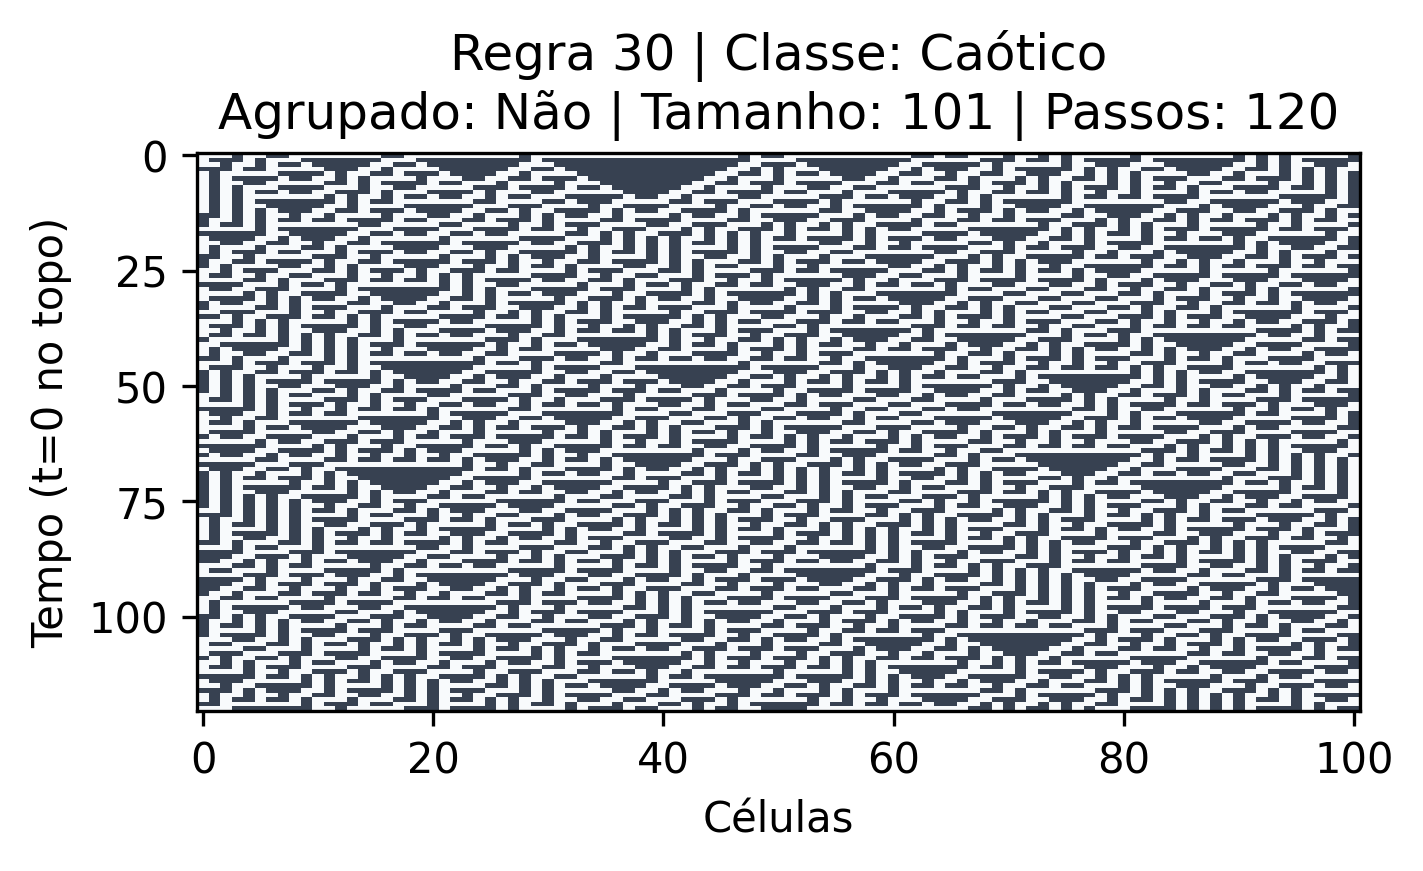
\includegraphics[width=0.75\textwidth]{figuras/resultados/regra_30_tamanho_101_passos_120_estado_aleatorio_densidade_0_8_agrupado_nao_classe_caotico.png}
    \caption{Regra 30 com densidade 0,8 (estado aleatório).}
    \label{fig:extra-r30-a08}
\end{figure}

\begin{figure}[H]
    \centering
    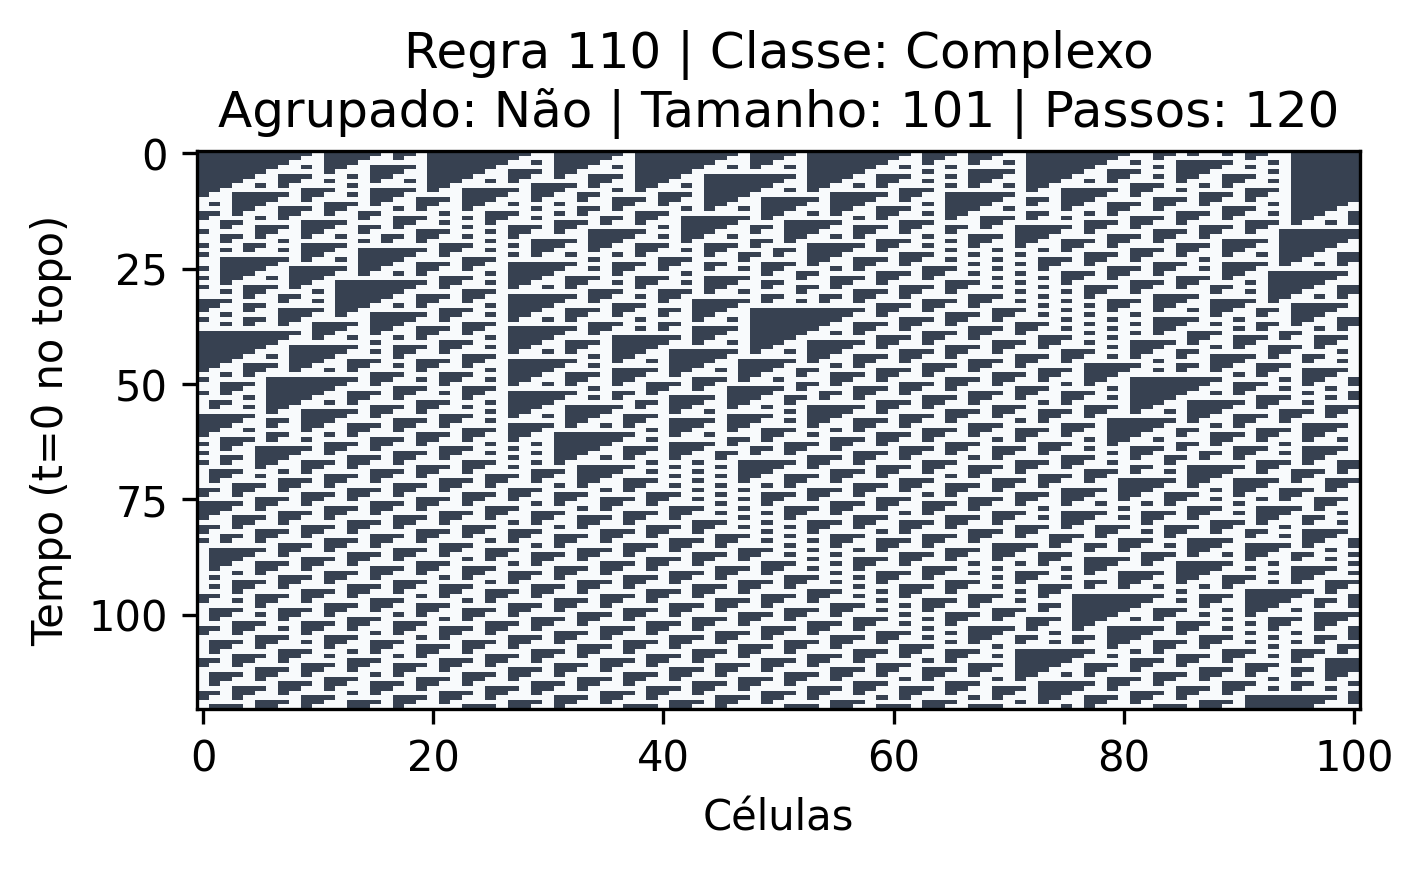
\includegraphics[width=0.75\textwidth]{figuras/resultados/regra_110_tamanho_101_passos_120_estado_aleatorio_densidade_0_2_agrupado_nao_classe_complexo.png}
    \caption{Regra 110 com densidade 0,2 (estado aleatório).}
    \label{fig:extra-r110-a02}
\end{figure}

\begin{figure}[H]
    \centering
    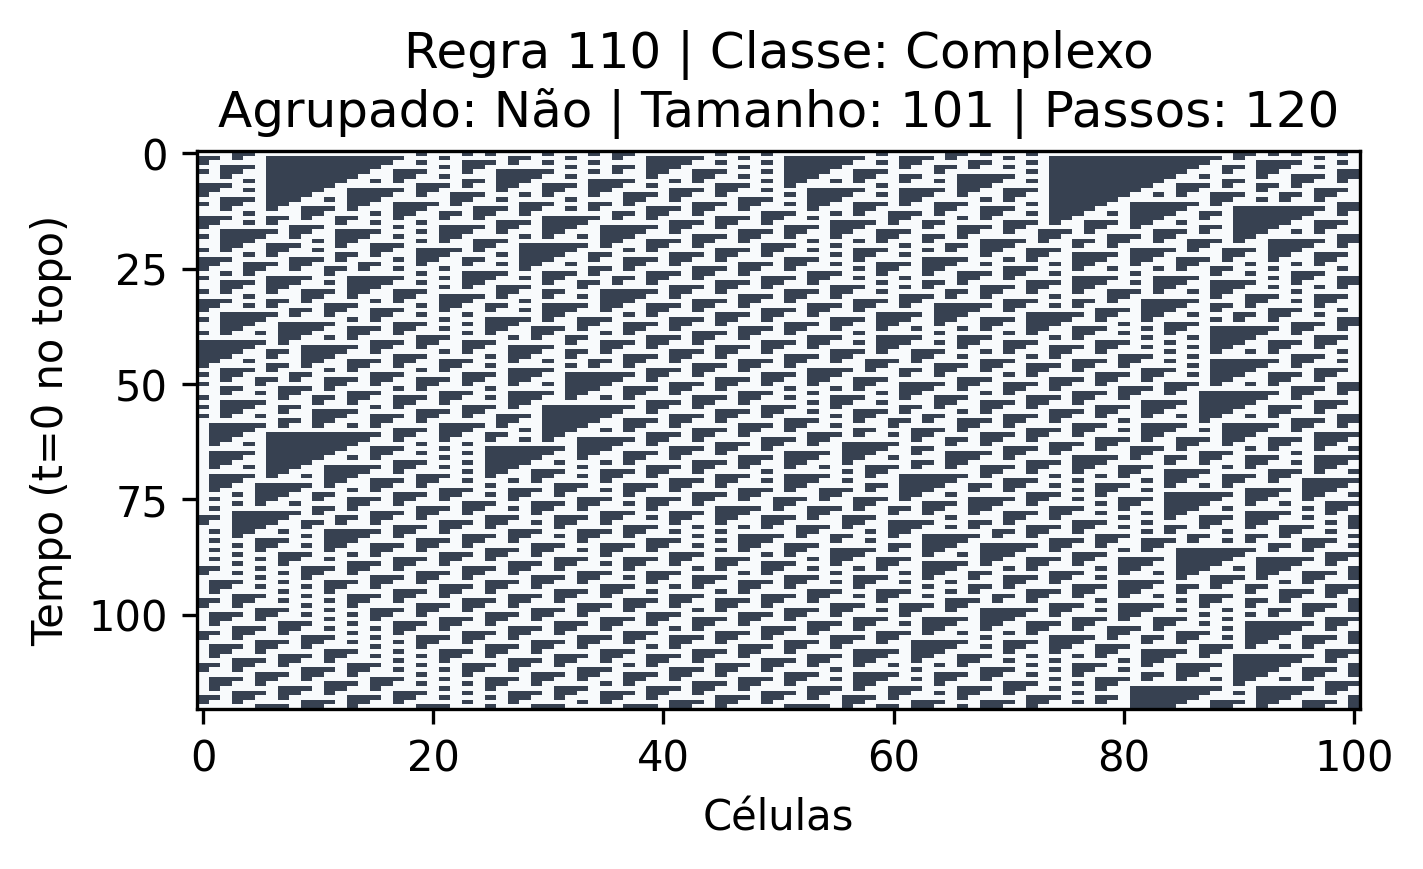
\includegraphics[width=0.75\textwidth]{figuras/resultados/regra_110_tamanho_101_passos_120_estado_aleatorio_densidade_0_8_agrupado_nao_classe_complexo.png}
    \caption{Regra 110 com densidade 0,8 (estado aleatório).}
    \label{fig:extra-r110-a08}
\end{figure}

Nas Figuras~\ref{fig:extra-r30-a02}, \ref{fig:extra-r30-a05} e \ref{fig:extra-r30-a08}, observa-se que a Regra 30 mantém comportamento globalmente irregular em diferentes densidades, com mudança clara na textura do padrão. Para a Regra 110, as Figuras~\ref{fig:extra-r110-a02} e \ref{fig:extra-r110-a08} evidenciam variação na organização espacial das estruturas propagantes conforme a ocupação inicial. Já as Figuras~\ref{fig:extra-r255-a05} e \ref{fig:extra-r108-a05} mostram que, mesmo com estado aleatório, as classes homogênea e periódica preservam suas características dominantes.

\section{Simulações com agrupado = sim}

As simulações com agrupado = sim, já realizadas no executável, foram incorporadas ao conjunto de resultados para explicitar o efeito de agrupamento da condição inicial aleatória, mantendo o recorte de \(tamanho=101\).

\begin{figure}[H]
    \centering
    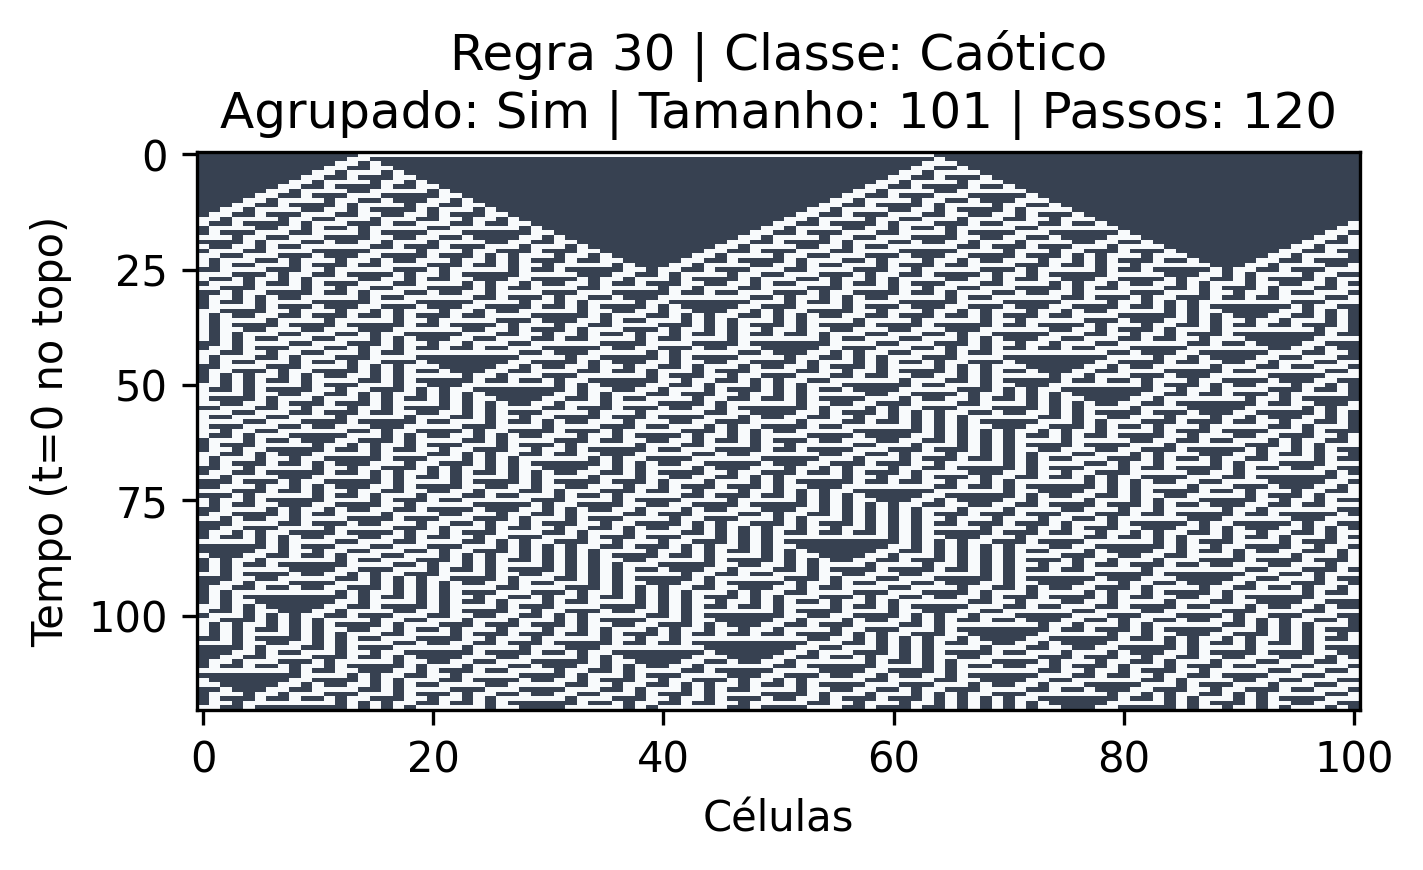
\includegraphics[width=0.75\textwidth]{figuras/resultados/regra_30_tamanho_101_passos_120_estado_aleatorio_densidade_0_5_agrupado_sim_classe_caotico.png}
    \caption{Regra 30 com estado aleatório, densidade 0,5 e agrupado = sim (tam101, passos120).}
    \label{fig:agrupado-sim-r30-a05}
\end{figure}

\begin{figure}[H]
    \centering
    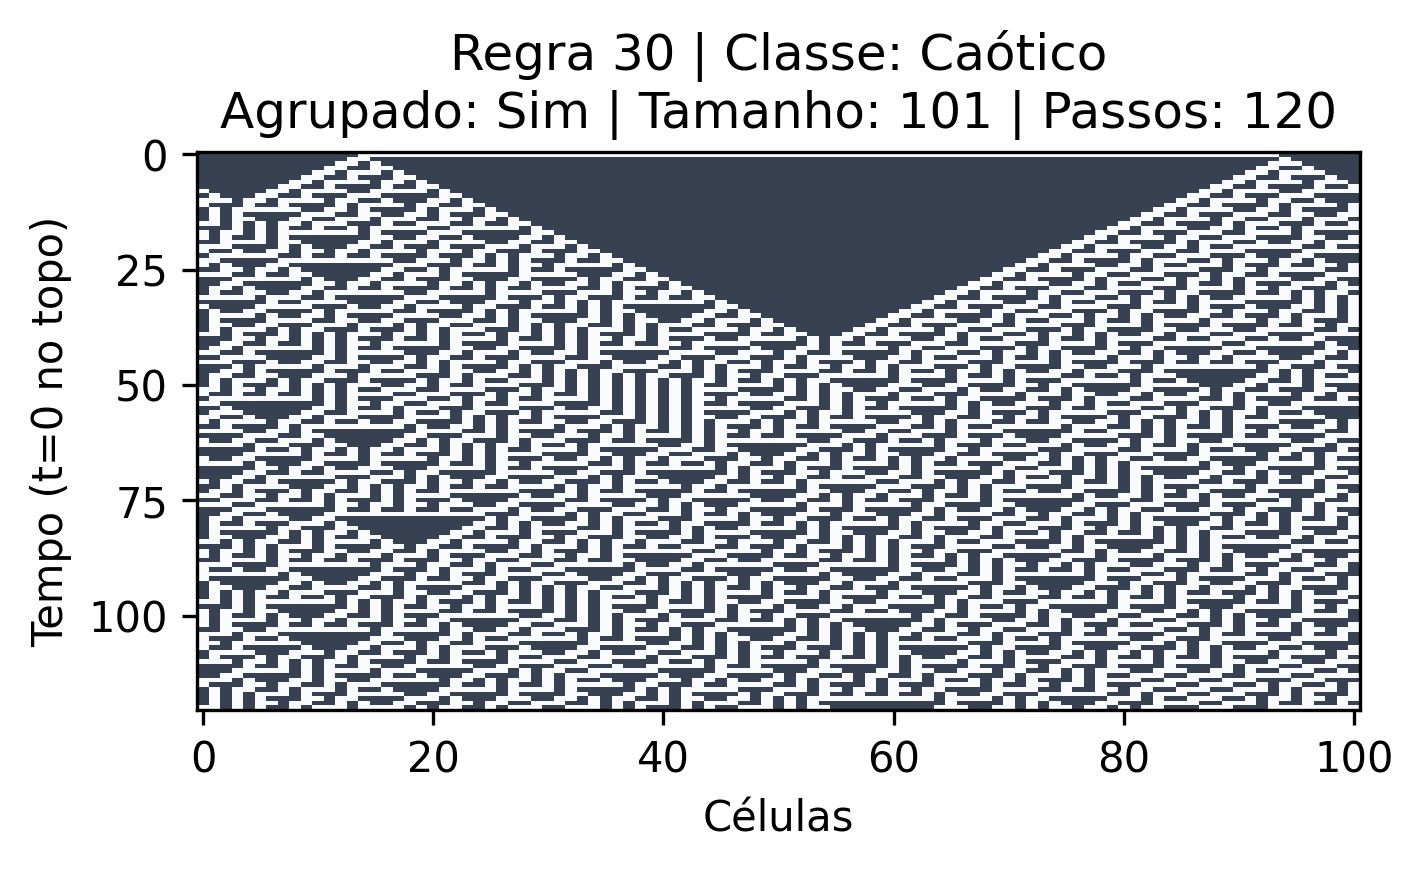
\includegraphics[width=0.75\textwidth]{figuras/resultados/regra_30_tamanho_101_passos_120_estado_aleatorio_densidade_0_8_agrupado_sim_classe_caotico.png}
    \caption{Regra 30 com estado aleatório, densidade 0,8 e agrupado = sim (tam101, passos120).}
    \label{fig:agrupado-sim-r30-a08}
\end{figure}

\begin{figure}[H]
    \centering
    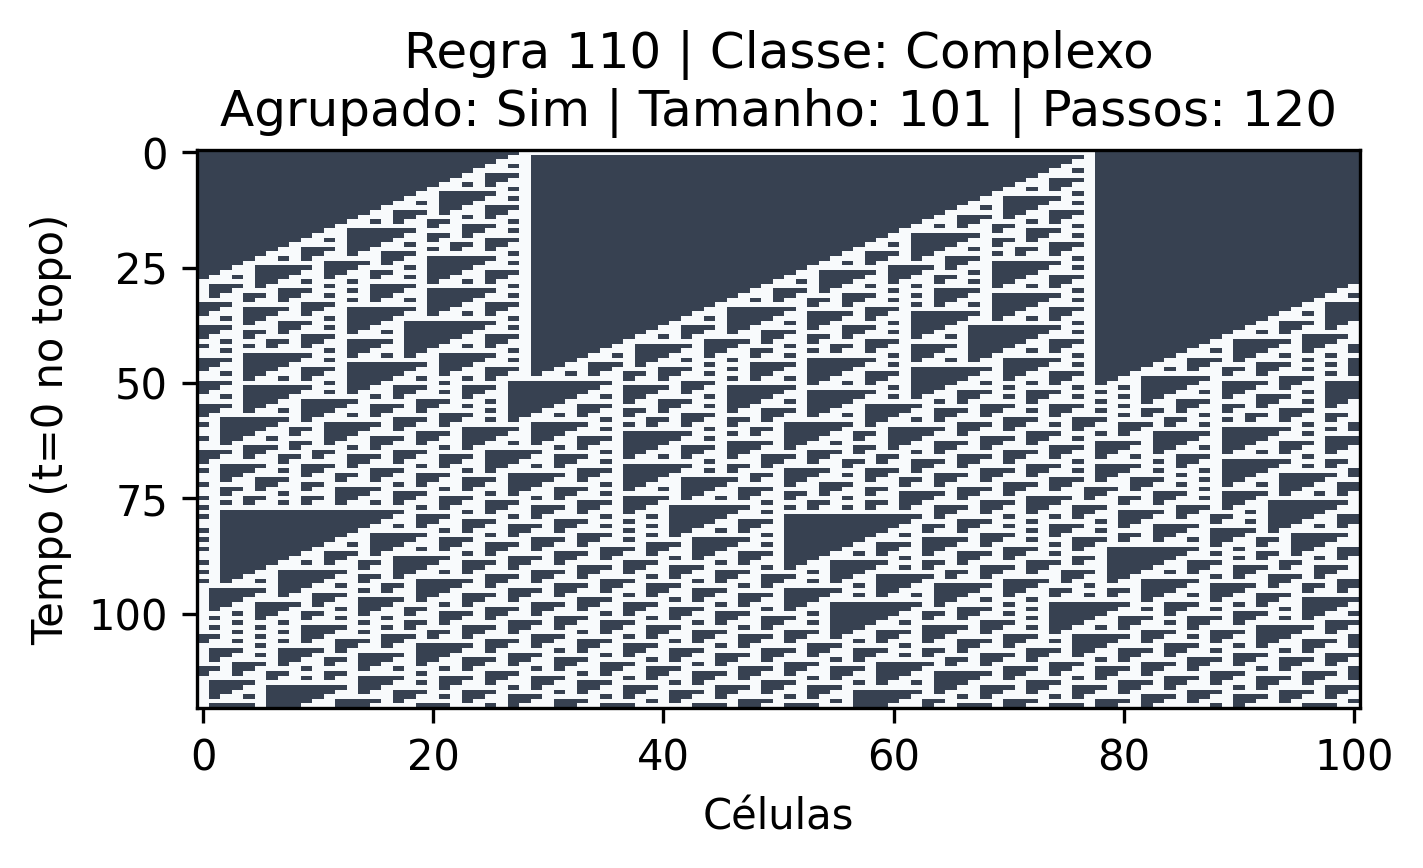
\includegraphics[width=0.75\textwidth]{figuras/resultados/regra_110_tamanho_101_passos_120_estado_aleatorio_densidade_0_5_agrupado_sim_classe_complexo.png}
    \caption{Regra 110 com estado aleatório, densidade 0,5 e agrupado = sim (tam101, passos120).}
    \label{fig:agrupado-sim-r110-a05}
\end{figure}

\begin{figure}[H]
    \centering
    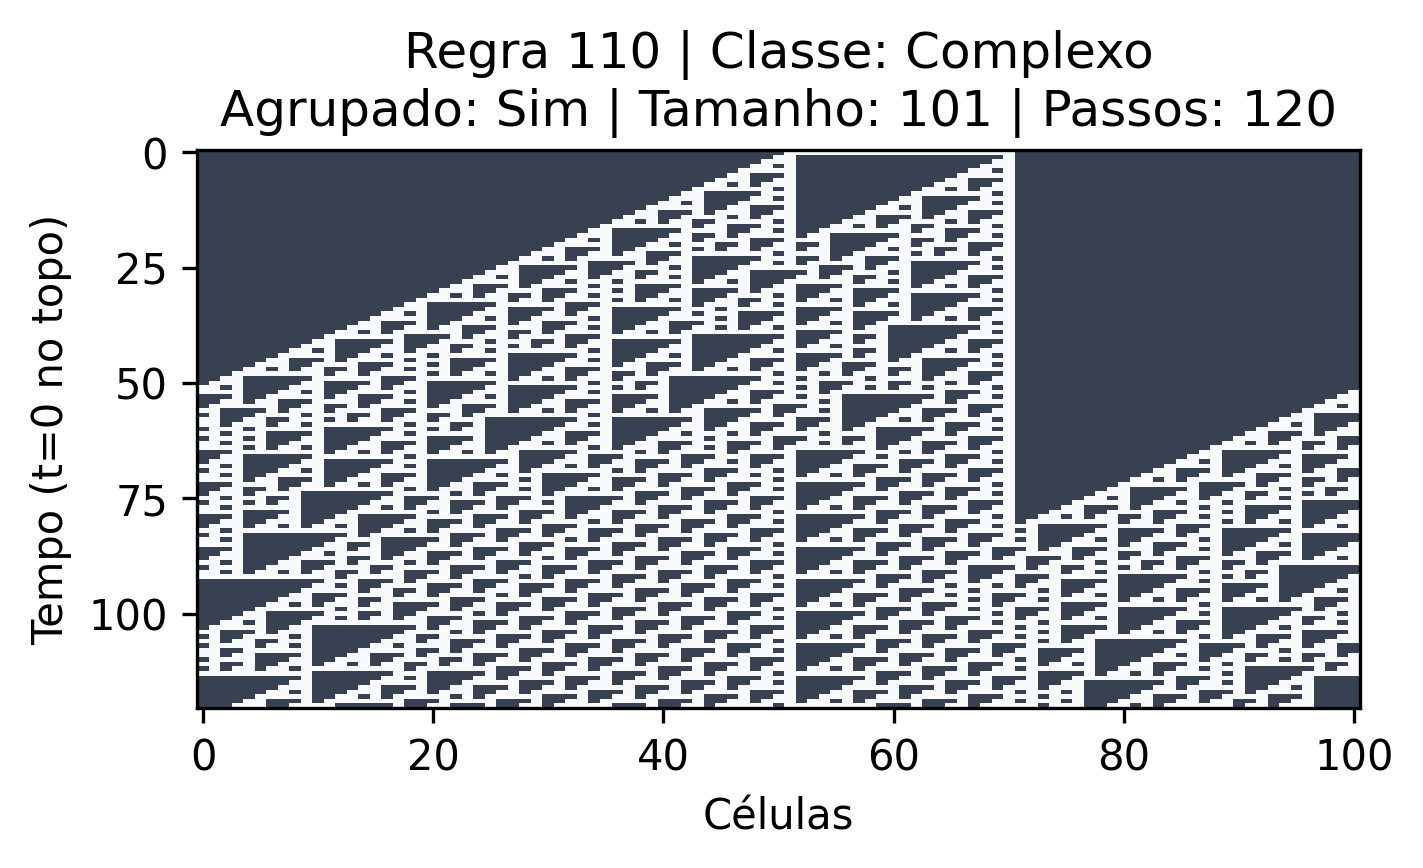
\includegraphics[width=0.75\textwidth]{figuras/resultados/regra_110_tamanho_101_passos_120_estado_aleatorio_densidade_0_2_agrupado_sim_classe_complexo.png}
    \caption{Regra 110 com estado aleatório, densidade 0,2 e agrupado = sim (tam101, passos120).}
    \label{fig:agrupado-sim-r110-a02}
\end{figure}

As Figuras~\ref{fig:agrupado-sim-r30-a05} e~\ref{fig:agrupado-sim-r30-a08} indicam que, para a Regra 30, o agrupamento inicial não elimina a dinâmica caótica, mas altera a formação de blocos e vazios nas primeiras iterações. De modo análogo, as Figuras~\ref{fig:agrupado-sim-r110-a05} e~\ref{fig:agrupado-sim-r110-a02} mostram que, para a Regra 110, o agrupamento modifica a distribuição inicial das estruturas sem descaracterizar o regime complexo.

Em síntese, os resultados apresentados neste capítulo mostram coerência entre os padrões observados e a classificação esperada das regras de Wolfram, além de evidenciar o efeito das condições iniciais e da densidade na evolução dos autômatos. O conjunto de figuras apresentado sustenta, de forma qualitativa, as conclusões discutidas para os diferentes regimes dinâmicos.

